\باب{بنیادی حقیقتونہ}
په دې باب کښ هغه خبرې راېوځاې کړې دې کومې به چه ټول کتاب کښ بېابېا رازې.امېد دې چه د کتاب لوستلو په وخت به په اصل مضمون باندې غور کول اسان وې.
\حصہ{بنیادی اکائی}
په دې کتاب کښ به د غونډې نړې اکائ نظام  استعمالېګې.په دے نظام کښ د تول اکائ کلوګرام، د ناپ اکائ مېټر،او د وخت اکائ سېکنډ دې 

\حصہ{مقداری او سمتیہ}
      
کہ د کراچئ نہ یو الوتکہ دشمال پہ مخ چھ سو ساټھ کلومیټر فی ګھنټہ روان وی نوھعہ بہ پہ دوہ ګھنټوکښ افعانستان کښ مزارشریف تہ اورسی۔پہ دے فقرہ کښ د الوتکےد رفتار مقداراو سمت دواړہ بیان کول ضروری دی۔داسے شے چہ ھعہ مقدار او سمت دواړہ لری، ھعے تہ سمتیہ وئیلی شی پہ دے مثال کښ سمتی رفتار تا سمتیہ دہ۔

دغہ رنګ کہ مونګ د دوہ کلوګرام دغنمو داوړو یا د شپږ لیټرو پټرولو خبرہ اوکو۔نو دے کښ دسمت ھیڅ ذکر نہ رازی ۔ھعہ شے چہ مقدار لری او سمت نہ لری ھعے تہ مقداری وئیلی شی ۔پہ دے مثال کښ وزن او حجم دواړہ مقداری دی۔
 
پہ دے کتاب کښ بہ مقداری شیزان د انګریزے یا لا طینے ژبے پہ سادہ لکھاے کښ پہ وړو حرفونو کښ یا پہ غټو حرفونو کښ لیکلی کیګی۔او پہ دے کتاب کښ سمتیہ شیزان د انګریزے یا لاطینے ژبے پہ غټہ لکھاے کښ پہ وړو حرفونو کښ یا پہ غټو حرفونو کښ لیکلے کیګی۔مثلا قوت د پارہ بہ ف استعمالیګی۔داسے سمتیہ چہ د ھعے اوږدوالے یو وی ھعے تہ اکائی سمتیہ وئیلی شی۔پہ دے کتاب کښ د انګریزے ژبے وړومبے وړوکے حرف چہ پہ غټہ  لکھاے کښ لیکلی وی اکائی سمتیہ پہ ګوتہ کوی۔ مثلا اکائی سمتیہ  ۱،۲،۳ د خلا درے ګوټونہ پہ ګوتہ کوی۔۱ کښ پہ وړہ لکھائی کښ ۱، دا د خلا ۱،طرف پہ ګوتی کوی۔کہ چرے د سمتیہ اوږدوالے او د ھعے مخ جداجدا لیکل وی نو د ھعے اوږدوالی پہ ګوتہ کولو د پارہ پہ سادہ لکھائی کښ ھعہ حرف استعمالیګی کوم چہ سمتیہ پہ ګوتہ کولو د پارہ پہ غټہ لکھائی کښ استعمال شوی ۔دا رنګے د سمتیہ ف اوږدوالے بہ ف لیکلے شی۔عکس کښ د سمتیہ ف اوږدوالے ف څلوردے۔کہ چرے د سمتیہ پہ سمت یو اکائی سمتیہ جوړہ کړے شی نو دا اکائی سمتیہ د ھعے سمتیے سمت ظاہروی۔دسمتیہ ف سمت بہ پہ اکائی سمتیہ ا ف لیکلے کیږی۔دلتہ پہ وړوکے لیک کښ  ف دا خبرہ څرګندہ کوی چہ دا اکائی سمتیہ د ف سمت ظاہروی۔پہ عکس کښ ا ف د ا ے برابر دہ ځکہ چہ د ف مخ ښی طرف تہ دے۔     
\begin{figure}
\centering
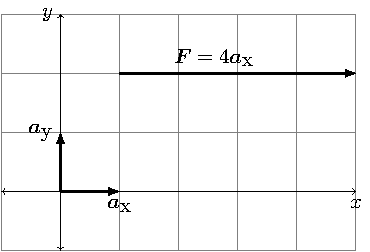
\includegraphics{figBasicFactsUnitVectors}
\caption{کارتیسی محدد}
\label{شکل_حقائق_اکائی_سمتیہ}
\end{figure}
\حصہ{محدد، خط مرتب}   
   دنیا درے ګوټہ دہ۔پہ دے کښ کہ ہرہ نقطہ واغستے شی نو د ھعے مقام پہ درے محدد ظاہرولے شی۔نورہ دا چہ پہ خلا کښ ہرہ سمتیہ،  یو بل تہ ولاړ د دریو اکائی سمتیو پہ امداد څرہ لیکلے شی۔راځی چہ د محدد یو څو قسمونہ اوګورو۔ 

\جزوحصہ{کارتیسی محدد} 
د خلا یو بل تہ ولاړ، درے اکائی سمتیہ پہ عکس کښ ښودلے شوی دی۔د یو بل تہ ولاړ مطلب دا دے چہ پہ دوی کښ ہر یو اکائی سمتیہ نورو دواړو تہ پہ نوی زاویہ دہ۔دہ دوی  سمت کښ اوږدوالے پہ ا،ب،ګ ظاہرولے شی۔  

   کہ چرے د خی لاس څلور ګوتے د الف د سمت طرف تہ اونیولے شی او بیا دا ګوتے د ب د سمت طرف تہ راتاو کړے شی نو د دے لاس کټہ ګوتہ بہ د ج سمت ظاہری۔دارنګے د خلا، یو بل تہ اولاړ، درے اکائی سمتو نظام د خی لاس نظام بوئی۔

پہ عکس کښ د مرکز نہ تر پ سمتیہ الف ښودلے شوے دہ۔پہ کارتیسی نظام کښ دغہ سمتیہ د دریو سمتیو  پہ مدد څرہ داسے لیکلے کیږی۔
\begin{align}
\kvec{A}=\kvec{A}_x+\kvec{A}_y+\kvec{A}_z
\end{align}
یا
\begin{align}
\kvec{A}=x\ax+y\ay+z\az
\end{align}
%
\begin{figure}
\centering
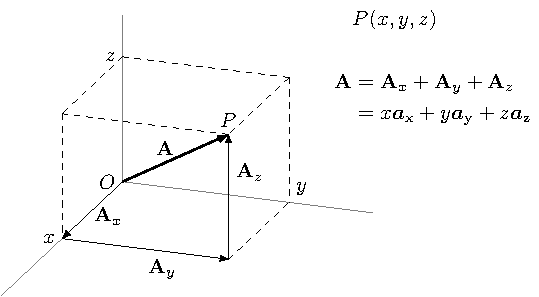
\includegraphics{figBasicFactsVectorCartesianCoordinates}
\caption{کارتیسی محدد نظام میں ایک سمتیہ}
\label{شکل_حقائق_کارتیسی_نظام_ایک_سمتیہ}
\end{figure}

کہ پہ کارتیسی نظام کښ ج صفر کیښودے شی او الف،ب بدلیږی نو مونږ تہ بہ الف ب سطح حاصلیږی۔کہ عکس کښ ف یو نقطہ وی او سطح الف ب مونږ زمکہ اوګنړو نو پہ عکس کښ د ډبی پہ پاسنے سطح د ج قیمت  پہ دریو ټکاو دے یعنی ز=۳خو الف د صفر نہ تر دریو پورے او ب د صفر نہ تر څلورو پورے قیمت لرلے شی۔دغہ رنګے د ډبی پاسنے سطح داسے لیکلے شی۔
\begin{align}
 \text{ڈبے کا بالائی سطح}= \left\{ 
  \begin{array}{l}
    0<x<2\\
    0<y<4 \\
	 z=3
  \end{array} \right.
\end{align}
کہ چرے د ج قیمت د صفر نہ تر دریو پورے، د الف قیمت د صفر نہ تر دوو پورے او د ب قیمت د صفر نہ تر څلورو پورے بدلیږی نو مونږ تہ بہ پہ عکس کښ د ښودلی ډبی حجم حاصل شی۔دغہ رنګ د دے ډبی حجم بہ  داسے لیکلے شی۔   
\begin{align}
 \text{ڈبے کاحجم}= \left\{ 
  \begin{array}{l}
    0<x<2\\
    0<y<4 \\
    0<z<3
  \end{array} \right.
\end{align}


\جزوحصہ{نلکی محدد}
 د مرکز نہ  تر نقطہ ف پورے سمتیہ الف پہ شکل کښ ښکاری۔دغہ سمتیہ پہ دوو سمتیو څرہ داسے لیکلے شی۔
\begin{align}
\kvec{A}=\kvec{\rho}+\kvec{A}_z
\end{align}
یا
\begin{align}
\kvec{A}=\rho \arho+z \az
\end{align}
%
\begin{figure}
\centering
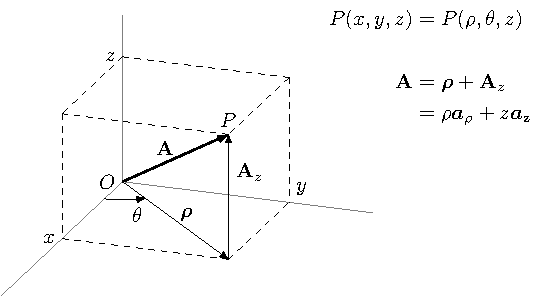
\includegraphics{figBasicFactsVectorCylindricalCoordinates}
\caption{نلکی محدد نظام}
\label{شکل_حقائق_نلکی_نظام_ایک_سمتیہ}
\end{figure}
 سمتیہ ف پہ الف ب سطح دہ۔د دے شکل نہ ښکارہ دہ چہ
\begin{align}
x&=\rho \cos \theta\\
y&=\rho \sin \theta
\end{align}
کہ چرے مونږہ د الف،ب،ج، پہ ځاے ز استعمال کو نو دغہ نقطہ داسے ہم لیکلے شو۔ھعہ نظام تہ چہ پہ کوم کښ د نقطے مقام ز سرہ ظاہرولے شی نلکی محدد وائی۔دلتہ عکس تہ اوګورے چہ کوم کښ د نلکی محدد، یو بل تہ ولاړ، درے اکائی سمتیے ښودلے شوی دی۔دا نظام ھم د خی لاس  نظام دے۔کہ چرے د خی لاس څلور ګوتے د الف د سمت طرف تہ اونیولے شی او بیا دا څلور ګوتے د ب د سمت طرف تہ راتاو کړے شی نو د دے لاس کټہ ګوتہ بہ د ج سمت ظاہرئی۔رازے چہ د دے دریو اکائی سمتیو تفصیل اولولو۔

کہ د الف،ب، سطح پہ مرکز، د محدد الف نہ پہ ب زاویہ اکائی سمتیہ جوړہ کړے شی نو دا بہ الف اکائی سمتیہ وی۔کہ ھم پہ دے الف،ب، سطح د مرکز نہ، زاویہ ډیریدو طرف تہ، الف اکائی سمتیہ تہ اولاړہ اکائی سمتیہ جوړہ کړے شی نو دا بہ ب اکائی سمتیہ وی۔پہ دے نظام کښ ف اکائی سمتیہ ھم ھعہ دہ چہ کوم کارتیسی نظام کښ وی۔دا یاد ولرے چہ پہ نلکی نظام کښ د الف او ب سمتونہ ځاے پہ ځاے بدل وی۔دا حقیقت پہ عکس کښ ښودلے شوے دے۔
\begin{figure}
\centering
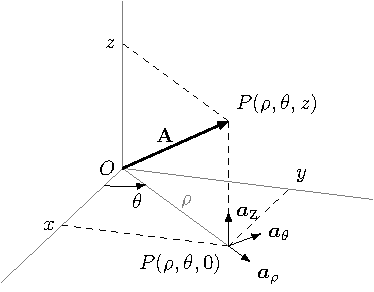
\includegraphics[height=3.5cm]{figBasicFactsCylindricalCoordinates}
\caption{نلکی نما محدد کی تعریف}
\label{شکل_حقائق_نلکی_نظام_تعریف}
\end{figure}
څنګہ چہ پہ عکس کښ ښودلے شوے دی، کہ چرے نلکی محدد کښ یو سمتیہ جوړہ کړے شی چہ $z$ یے صفر وی، د رداس قیمت یے ټکاو وی او زاویہ د صفر نہ $2\pi$ پورے بدلہ کړے شی نو د دے سمتیے سر بہ پہ $x-y$ سطح باندے چورلندے دائرہ راخکی۔کہ چرے د دغے سمتیے $z$ ھم بدل کړے شی، نو دا سمتیہ بہ د دروځے عکس جوړ کی۔پہ دے وجہ دے نظام تہ  د نلکی محدد نظام وائی۔اس کہ چرے د دے سمتیے  رو،تھیټا او ز بدل کړے شی نو مونږ تہ بہ نلکی حجم ملاو شی۔دا درے خبرے  داسے لیکلے شی۔
\begin{align}
 \text{دائرہ}&= \left\{ 
  \begin{array}{l}
    \rho=\rho_0\\
    0<\theta<2 \pi \\
    z=0
  \end{array} \right.
\end{align}
%
\begin{align}
 \text{نلکی نما سطح}&= \left\{ 
  \begin{array}{l}
    \rho=\rho_0\\
    0<\theta<2 \pi \\
  0<z<z_0
  \end{array} \right.
\end{align}
%
\begin{align}
 \text{نلکی کا حجم}= \left\{ 
  \begin{array}{l}
    0<\rho<\rho_0\\
    0<\theta<2 \pi \\
  0<z<z_0
  \end{array} \right.
\end{align}
%
\begin{figure}
\centering
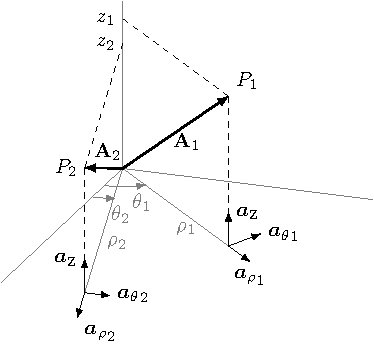
\includegraphics[height=3.5cm]{figBasicFactsCylindricalCoordinatesVaryingUnitVectors}
\caption{نلکی محدد میں اکائی سمتیہ \عددیء{\arho} اور \عددیء{\atheta} ہر نقطہ پر مختلف ہیں۔}
\label{شکل_حقائق_نلکی_نظام_میں_اکائی_سمتیات_اٹل_نہیں}
\end{figure}
%
\begin{figure}
\centering
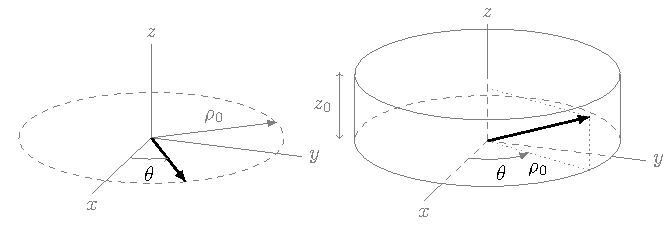
\includegraphics[height=2.5cm]{figBasicFactsCylindricalCoordinatesCircleAndCylinder}
\caption{‫نلکی محدد میں دائرہ اور نلکی‬}
\label{شکل_حقائق_نلکی_نظام_میں_دائرہ_اور_نلکی}
\end{figure}


\حصہ{سمتی رقبہ}
دلتہ عکس باندے نظر ساتے۔کہ چرے سطح تہ ولاړہ  اکائی سمتیہ جوړہ کړے شی نو دا اکائی سمتیہ بہ د سطح سمت ظاہری۔ہرہ سطح، مثلاً د کتاب  پانړہ،  دوہ مخہ لری، دا رنګے دہرے سطح دوہ سمتیے بیانیدے شی۔مسئلے تہ د کتلو نہ پس،پہ   دے دوو کښ یو د سطح سمت خوښ کړے شی۔خو کہ چرے دا سطح پورہ بند عکس لری، مثلاً پنډوس، نو بیا بہر طرف تہ اکائی سمتیہ د دے سطح سمت ښائی۔عکس الف پورہ بندہ سطح ښائی۔پہ دے عکس کښ د پاسنئی سطح رقبہ الف دہ او سمت ۓ  ز دے نو دغہ رنګے الف سمتیہ اوږدوالے الف لری او سمت ے ز دے۔ 
\begin{figure}
\centering
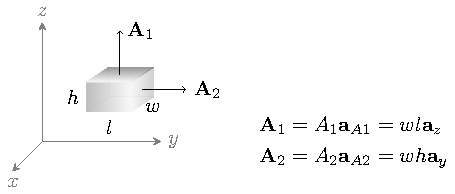
\includegraphics[height=2.5cm]{figBasicFactsVectorArea}
\caption{سمتیہ رقبہ کا تعارف‬}
\label{شکل_حقائق_رقبہ_سمتیہ}
\end{figure}
%
\begin{align*}
A_1&=wl\\
\kvec{a_{A1}}&=\az
\end{align*}
لہٰذا
\begin{align}
\kvec{A_1}=A_1 \kvec{a_{A1}}= w l \az
\end{align}
کہ پہ عکس الف کښ د خی مخ خبرہ اوکړو نو د دے سمتیہ سمت  الف دے او د دے اوږدوالے ب دے۔
\begin{align*}
A_2=wh\\
\kvec{a_{A2}}=\ay
\end{align*}
لہٰذا
\begin{align}
\kvec{A_2}=A_2 \kvec{a_{A1}}=w h \ay
\end{align}
پہ دغہ عکس کښ د لاندینئی سطح رقبہ الف دہ او د دے سمت د الف الوړے دے نو دا رنګ مونګ لیکلے شو  
\begin{align}
\kvec{A_3}=A_3 \kvec{a_{A3}}=wl (-\az)=-wl \az
\end{align}

د سمتیے اوږدوالے چرے ھم منفی نہ شی کیدے خو د دے سمت مثبت یا منفی کیدے شی نو ځکہ د سمتی رقبہ سمت مثبت یا منفی کیدے شی خو اوږدوالے یے منفی نہ شی کیدے۔


\حصہ{رقبہ د ولاړ تراش}
کہ د یو څیز اوږدوالی تہ ولاړہ کرخہ  باندے دا څیز پرے کړے شی نو دے تہ ولاړ تراش ویلے شی۔  

پہ عکس الف کښ یوہ لختہ د ے سمت کے ملاستہ  دہ۔کہ مونږ پہ تصور کے پہ دے لختہ ولاړ تراش ولګو نو د لختے د پریکړے مخ رقبے تہ د ولاړ تراش رقبہ وئلے شی۔پہ دے عکس کے د ولاړ تراش سمتی رقبہ الف او سمت ے الف دے۔
\begin{align}
A=wh
\end{align}
%
\begin{align}
\kvec{a_A}=\ay
\end{align}
پہ دغہ عکس کښ د لختے ګس سر تہ الف او ب ښودلے شوی دی۔دغلتہ پہ ګول دائرہ کښ بندہ نقطہ وھلے شوے دہ۔ ګول دائرہ کښ بندہ نقطہ، د کتاب پانړے تہ ولاړہ، د لوستونکی طرف تہ اکائی سمتیہ ښائی۔دلتہ دغہ الف اکائی سمتیہ دہ۔د دے اکائی سمتیے اړولے طرف، لکہ د کتاب  پانړے تہ ولاړ لاندے مزکے طرف تہ اکائی سمتیہ پہ ګول دائرہ کښ بند صلیب سرہ ظاھرولے شی۔
\begin{figure}
\centering
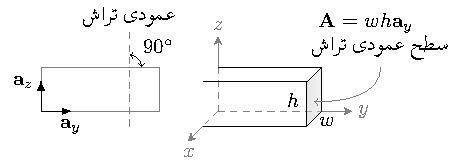
\includegraphics[height=2.5cm]{figBasicFactsCrossSectionalArea}
\caption{رقبہ  عمودی تراش}
\label{شکل_حقائق_رقبہ_عمودی}
\end{figure}


\حصہ{برقی میدان او مقناطیسی میدان}    
\جزوحصہ{برقی میدان اود برقی میدان تاو}
  د کولمب قانون وائی چہ د دوو چارج شوے څیزونو تر مینځ د یو بل راښکلو قوت یا د یو بل ټیلہ کولو قوت د دوو چارجو حاصل ضرب پہ نسبت وی او دہ فاصلے د مربع د نسبت الټہ وی۔دواړہ چارجونہ بالکل یو شانتے قوت محسوس کوی۔دا رنګے کہ چارج الف د دریو نیوټنو قوت ټیلہ محسوس کوی نو چارج ب بہ ھم د دریو نیوټنو قوت ټیلہ محسوس کوی۔کہ د دوو چارجونو تر مینځ نیغہ کرښہ راښکلے شی، نو پہ دوئی بہ د قوت سمت ھم پہ دے کرخہ وی۔  
\begin{align}\label{مساوات_بنیادی_کولمب_کا_قانون}
F=\frac{q_1 q_2}{4 \pi \epsilon r^2}
\end{align}
کہ د یو پروت چارج خوا تہ یو دویم چارج راوستے شی نو دی دواړہ بہ قوت راښکل یا قوت ټیلہ محسوس کوی۔د دے قوت قیمت د کولمب قانون سرہ حاصلول شی۔دویم چارج چہ کوم قوت محسوس کوی، مونږ پہ دے نظر ږدو۔ دا دویم چارج چہ د وړومبی چارج نہ څومرہ لرے بوتلے شی، دے دومرہ کم قوت محسوس کوی۔پہ لرے بوتلو بوتلو آخر د دوی تر مینځہ فاصلہ دومرہ ډیرہ شی چہ قوت د محسوس کیدو د حد نہ ھم کم شی۔مونږ وایو چہ دا دویم چارج د وړومبی چارج د زور نہ باہر شو۔

د چارج چارچاپیرہ، تر کومے چہ د دے اثر محسوس کیدے شی، دغہ  علاقے تہ  برقی میدان وئیلے شی۔

برقی میدان د یو یا د یو نہ ډیرو چارجونو د لاسہ پیدا کیدے شی۔

برقی میدان کښ پروت اکائی مثبت چارج باندے قوت تہ د برقی میدان تاو وئیلے شی۔

د برقی میدان تاو اکائی وولټ فی میټر دہ۔

   رازے چہ د کولومب قانون یعنی مساوات الف  سرہ د چارج ق د برقی میدان تاو حاصل کړو۔د ق چارج میدان کښ   پہ اکائی مثبت چارج  باندے قو
\begin{align}
F=\frac{Q \times 1}{4 \pi \epsilon r^2}=\frac{Q}{4\pi\epsilon r^2}
\end{align}
وی۔ھم دغے تہ د میدان تاو وائی۔
\begin{align}
E=\frac{Q}{4\pi\epsilon r^2}
\end{align}


\ابتدا{مثال}
سوال:پہ برقی میدان کښ پروت څلور کولومب چارج د جنوب سمت تہ د شل نیوټن قوت محسوس کوی۔د دے برقی میدان تاو حاصل کړے۔

حل:چہ پہ څلوو کولومب باندے شل نیوټن قوت وی نو پہ اکائی چارج بہ پینځہ نیوټن قوت وی او دا قوت بہ ھم د جنوب سمت کښ وی۔دغہ رنګ د برقی میدان تاو د جنوب سمت کښ پینځہ وولټ فی میټر دے۔
\انتہا{مثال} 

\جزوحصہ{مقناطیسی میدان او د مقناطیسی میدان تاو}
مقناطیسی میدان او د مقناطیسی میدان تاو بالکل د برقی میدان او د برقی میدان تاو پہ شان وی۔

کہ د یو پروت مقناطیس خوا تہ یو دویم مقناطیس راوستے شی نو دی دواړہ بہ قوت راښکل یا قوت ټیلہ محسوس کوی۔دویم مقناطیس چہ کوم قوت محسوس کوی، مونږ پہ دے نظر ږدو۔ دا دویم مقناطیس چہ د وړومبی مقناطیس نہ څومرہ لرے بوتلے شی، دے دومرہ کم قوت محسوس کوی۔پہ لرے بوتلو بوتلو آخر د دوی تر مینځہ فاصلہ دومرہ ډیرہ شی چہ قوت د محسوس کیدو د حد نہ ھم کم شی۔مونږ وایو چہ دا دویم مقناطیس د وړومبی مقناطیس د زور نہ باہر شو۔

د مقناطیس چارچاپیرہ، تر کومے چہ د دے اثر محسوس کیدے شی، دغہ  علاقے تہ مقناطیسی میدان وئیلے شی۔

مقناطیسی میدان د یو یا د یو نہ ډیرو مقناطیسونو د لاسہ پیدا کیدے شی۔

پہ کائنات کښ د مقناطیس شمال او جنوب قطب تل جوړہ پائی۔چرے ھم شمال یا جنوب قطب یوازے نہ دی موندلے شوے۔بیا ھم کہ چرے مونږ یو فرضی شمال قطب پہ مقناطیسی میدان کښ کیږدو نو دا قطب بہ قوت محسوس کوی۔ 

مقناطیسی میدان کښ پروت اکائی شمال قطب باندے قوت تہ د مقناطیسی میدان تاو وئیلے شی۔

\حصہ{سطحی او حجمی کثافت}
کہ یو څیز پہ یو سطح ہر ځاے یو شانتے خور وی نو پہ دے صورت کښ پہ اکائی رقبہ کښ د دے څیز مقدار تہ د دغہ څیز سطحی کثافت وئیلے شی۔حقیقت کښ عموماً یو څیز ہر ځاے کښ یو شانتے خور نہ وی، پہ دے صورت کښ کہ  کل  رقبہ الف وی او پہ دے ټولہ رقبہ د  دے څیز کل مقدار ب وی نو د دے څیز اوسط سطحی کثافت بہ 
\begin{align}
B_{\textup{اوسط}}=\frac{\phi}{A}
\end{align}
وی۔دا مساوات داسے ھم لیکلے شی۔
\begin{align}
\phi=B_{\textup{اوسط}} A
\end{align}

داسے کہ چرے د یو بدلیدونکی څیز سطحی کثافت معلوم وی نو د دغہ څیز کل مقدار پہ دغہ سطح مساوات الف سرہ حاصلیدے شی۔

 کہ چرے یو څیز پہ یو سطح ځاے پہ ځاے  یو شانتے خور نہ وی نو پہ دے صورت کښ کہ مونږ یو دومرہ وړہ رقبہ واخلو چہ پہ دے کښ ہر ځاے کښ دغہ څیز یو شانتے خور ګنړلے شی نو پہ دے صورت کښ پہ دغہ وړہ سطح باندے  سطحی کثافت بہ
\begin{align}
B=\frac{\Delta \phi}{\Delta A}
\end{align}

وی چہ کوم ځاے الف دا وړہ رقبہ او ب پہ دے کښ د دغہ څیز کل مقدار دے۔کہ چرے دا وړہ رقبہ د نقطے پہ شان وړہ کړے شی نو پہ دے صورت کښ پہ دے نقطے باندے د نقطے سطحی کثافت داسے لیکلے شی۔
\begin{align}
B=\frac{\dif \phi}{\dif A}
\end{align}
دا مساوات مونږ داسے  ھم لیکلے شو
\begin{align}
\dif \phi =B \dif A
\end{align}
دغہ رنګ کہ چرے مونږ تہ پہ یو نقطہ باندے د نقطے سطحی کثافت معلوم وی نو پہ دے نقطہ د څیز کل مقدار د مساوات الف پہ مدد حاصلیدے شی۔ 

داسے کہ پہ یو تار کښ برقی رو الف وی او د دے تار عمودی تراش رقبہ ب وی نو پہ دے تار کښ د برقی رو اوسط کثافت بہ 
\begin{align}\label{مساوات_بنیادی_برقی_رو_کثافت}
\rho_{\textup{اوسط}}=\frac{I}{A}
\end{align}
وی۔

\جزوحصہ{حجمی کثافت} 
 اکائی حجم کښ د یو څیز مقدار تہ د ھعہ څیز حجمی کثافت وائی۔مثلاً کہ  یو څیز الف وزن او ب حجم لری نو د دہ اوسط حجمی کثافت بہ پ وی۔کہ یو حجم کښ ځاۓ پہ ځاۓ د مادے مقدار یو شان نہ وی نو پہ دے صورت کښ پہ یو نقطہ حجمی کثافت حاصلولو د پارہ  پہ دغہ نقطے  دومرہ وړوکے حجم  واغستے شی چہ پکښ ہر ځاۓ د مادے مقدار یو شان ګنړل ممکن وی۔کہ پہ دے وړوکی حجم الف  کښ د مادے وزن ب وی نو پہ دے نقطے حجمی کثافت بہ پ وی۔
\begin{align}
\rho_{\textup{واسط}}=\frac{m}{V}
\end{align}
کہ چرے دا وړوکے حجم واقعی د نقطے مانند کړے شی نو بیا مونږ لیکلے شو 
\begin{align}
\rho=\frac{\dif m}{\dif V}
\end{align}
دغہ رنګے کہ مونږ تہ د نقطے حجمی کثافت معلوم وی نو مونږ د مساوات  الف پہ مدد سرہ دغلتہ وزن حاصلولے شو۔
\begin{align}
\dif m=\rho \dif V
\end{align}
 
\حصہ{صلیبی ضرب او د نقطے ضرب}
د دوو مقداری حاصل ضرب ھم مقداری وی۔د دے پہ ځاۓ  د دوو سمتیو حاصل ضرب سمتیہ او مقداری ممکن دہ۔د ضرب پہ دے قسمونو لږ غور کوو۔

\جزوحصہ{صلیبی ضرب}
کہ چرے د دوو سمتیو حاصل ضرب ھم سمتیہ وی نو داسے ضرب تہ صلیبی ضرب وئیلے شی۔صلیبی ضرب داسے لیکلے شی۔
\begin{align}
\kvec{C}=\kvec{A} \times \kvec{B}
\end{align}
صلیبی ضرب کښ د ضرب نخہ د صلیب شکل لری۔د صلیبی ضرب نوم ھم د دغے نخے نہ اغستے شوے دے۔

د الف سمتیے مقدار 
\begin{gather}
\begin{aligned}\label{مساوات_بنیادی_ضرب_صلیبی_تعریف}
C=\abs{\kvec{C}} &= \abs {\kvec{A}} \abs{\kvec{B}} \sin \theta_{AB}\\
&=A B \sin \theta_{AB}
\end{aligned}
\end{gather}
دے، کوم ځاۓ چہ د الف او ب سمتیو تر مینځ زاویہ د پ برابر دہ۔
\ابتدا{مثال}
درکړے شوے ضرب صلیبی حاصل کړے۔
\begin{itemize}
\item
$\ax \times \ay \quad \ay \times \az \quad \az \times \ax \quad \ax \times \az$ \\
\item
 $\az \times \ay \quad \ay \times \ay \quad \arho \times \atheta \quad \az \times \arho$
\end{itemize}


حل:پہ دے مثال کے تمام سمتیے اکائی سمتیے دی۔د اکائی سمتیے طول د یو برابر وی۔دا شان مونګ لیکلے شو
\begin{itemize}
\item
$\ax \times \ay=(1)(1) \sin 90 \az =\az$\\
\item
$\ay \times \az=(1)(1) \sin 90 \ax =\ax$\\
\item
$\az \times \ax=(1)(1) \sin 90 \ay =\ay$\\
\item
$\ax \times \az=(1)(1) \sin 90 (-\ay) =-\ay$\\
\item
$\az \times \ay=(1)(1) \sin 90 (-\ax) =-\ax$\\
\item
پہ دے مثال کے دواړہ سمتیے پہ یو سمت کے دی۔دا شان د دوی ترزامن زاویہ د صفر برابر دہ۔اس  \عددیء{\sin 0=0} وی نو داسے د صلیبی ضرب د صفر برابر دے۔
$\ay \times \ay=(1)(1) \sin 0  =0$\\
\item
$\arho \times \atheta=(1)(1) \sin 90  \az =\az$\\
\item
$\az \times \arho=(1)(1) \sin 90 \atheta =\atheta $\\
\end{itemize}
\انتہا{مثال}
%
\ابتدا{مثال}

پہ شکل \حوالہ{شکل_حقائق_کارتیسی_مروڑ_کا_حل} کے سلور نیوٹن قوت \سمتیہ{F} د محور سے تیننہ درے میٹر پہ سمتی فاصلہ \سمتیہ{L}  لاگو دے۔د دے قوت مروړ حاصل کړے۔

	حل:
د مروڑ \سمتیہ{T} تعریف دا دے
\begin{align}
\kvec{T}=\kvec{L} \times \kvec{F}
\end{align}
پہ کارتیسی نظام کے دا سمتی فاصلہ داسے لیکلے شی
\begin{align}
\kvec{L}=L \sin \theta \ax-L \cos \theta \ay
\end{align}
لہٰذا
\begin{align*}
\kvec{T}&=\left(L \sin \theta \ax-L \cos \theta \ay \right) \times F \ay\\
&=L \sin \theta \ax \times F \ay-L \cos \theta \ay \times F \ay\\
&= L F \sin \theta \az
\end{align*} 
دلتہ د تیر مثال پہ مدد سرہ \عددیء{\ax \times \ay=\az} او \عددیء{\ay \times \ay=0} اغستے شو۔ داسے
\begin{align*}
\kvec{T}= L F \sin \theta \az=12 \sin \theta \az \quad \si{\newton \meter}
\end{align*}
حاصلیګی۔پہ دے مثال کے \عددیء{\theta_{LF}=180\degree-\theta} دہ۔ د  زاویہ \عددیء{\alpha}   دپارہ \عددیء{\sin \alpha=\sin(180\degree-\alpha)} وی لہٰذا دغہ مروړ داسے ہم لیکلے شے
\begin{align*}
\kvec{T}&=LF\sin \theta \az\\
&=L F \sin \theta_{LF}\az
\end{align*}
ہم دغہ جواب د ضربِ صلیبی دہ تعریف یعنی مساوات \حوالہ{مساوات_بنیادی_ضرب_صلیبی_تعریف} او د خی لاس قانون سرہ زیات پہ آسانے حاصلیدے شی۔
\انتہا{مثال}
\begin{figure}
\centering
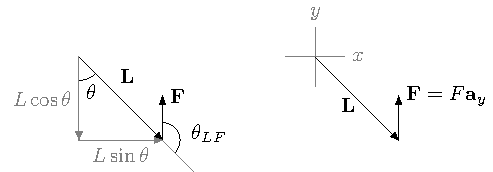
\includegraphics[height=2.5cm]{figBasicFactsVectorCrossProduct}
\caption{کارتیسی نظام میں مروڑ کا حل}
\label{شکل_حقائق_کارتیسی_مروڑ_کا_حل}
\end{figure}
%
\جزوحصہ{د نقطے ضرب}
کہ چرے د دوو سمتیو حاصل ضرب مقداری وی نو داسے ضرب تہ د نقطے ضرب وائی۔د نقطے ضرب داسے لیکلے شی۔
\begin{align}
\kvec{C}=\kvec{A} \cdot \kvec{B}
\end{align}
د نقطے ضرب کښ د ضرب نخہ د نقطے شکل لری۔د نقطے ضرب نوم ھم د دغے نخے نہ اغستے شوے دے۔

د الف سمتیے مقدار
\begin{gather}
\begin{aligned}\label{مساوات_بنیادی_ضرب_نقطہ_تعریف}
\kvec{C}&=\kvec{A} \cdot \kvec{B}\\
&=\abs{\kvec{A}} \abs{\kvec{B}} \cos \theta_{AB}\\
&=A B \cos \theta_{AB}
\end{aligned}
\end{gather}
دے، کوم ځاۓ چہ د الف او ب سمتیو تر مینځ زاویہ د پ برابر دہ۔

\ابتدا{مثال}
درکړے شوے ضرب نقطہ حاصل کړے۔

\begin{itemize}
\item
$\ax \cdot \ax \quad \ay \cdot \ay \quad \az \cdot \az$\\
\item
$\ax \cdot \ay \quad \ay \cdot \az \quad \arho \cdot \arho \quad \arho \cdot \atheta$
\end{itemize}

حل:دے مثال کے تمام اکائی سمتیے دی۔د اکائی سمتیے طول د یو برابر وی۔
\begin{itemize}
\item
$\ax \cdot \ax =(1) (1) \cos 0=1$\\
\item
$\ay \cdot \ay =(1) (1) \cos 0=1$\\
\item
$\az \cdot \az =(1) (1) \cos 0=1$\\
\item
$\ax \cdot \ay =(1) (1) \cos 90\degree=0$\\
\item
$\ay \cdot \az =(1) (1) \cos 90\degree=0$\\
\item
$\arho \cdot \arho =(1) (1) \cos 0=1$\\
\item
$\arho \cdot \atheta =(1) (1) \cos 90\degree=0$\\
\end{itemize}
\انتہا{مثال}
%
\ابتدا{مثال}
پہ شکل \حوالہ{شکل_حقائق_کارتیسی_کام}  کښ قوت \سمتیہ{F} یو بار ټیلا کوی۔د سمتی فاصلہ  \سمتیہ{L} طے  کولو باندے بہ قوت سمرہ کار کړے وی۔

	حل:
	د کار   \عددیء{W} تعریف دا دے
\begin{align}
W=\kvec{F} \cdot \kvec{L}
\end{align}
پہ ہم کارتیسی نظام کښ سمتی فاصلہ داسے لیکلے شی
\begin{align}
\kvec{L}=L \cos \theta_{FL} \ax +L \sin \theta_{FL} \ay
\end{align}
لہٰذا
\begin{gather}
\begin{aligned}
W &= (F \ax) \cdot (L \cos \theta_{FL} \ax +L \sin \theta_{FL} \ay)\\
&=F L \cos \theta_{FL} (\ax \cdot \ax)+ F L \sin \theta_{FL} (\ax \cdot \ay)\\
&= F L \cos \theta_{FL}
\end{aligned}
\end{gather}
%
\begin{figure}
\centering
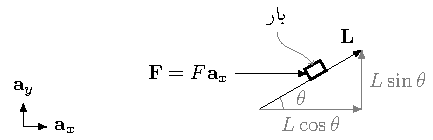
\includegraphics[height=2.5cm]{figBasicFactsWorkAsDotProduct}
\caption{کارتیسی نظام میں کام}
\label{شکل_حقائق_کارتیسی_کام}
\end{figure}
مونګ د تیر مثال پہ مدد سرہ  \عددیء{\ax \cdot \ax=1} او \عددیء{\ax \cdot \ay=0} اغستے دی۔ ہم دغہ جواب د  ضربِ نقطہ  تعریف یعنی مساوات \حوالہ{مساوات_بنیادی_ضرب_نقطہ_تعریف} سرہ زیان آسانے سرہ حاصلیدے شو۔
\انتہا{مثال}

\حصہ{شرحِ فرق}
مساوات الف کښ د کارندہ ب شرح فرق ښودلے شوے دے چہ د پکښ نہ بدلیدونکے جزو دے او مساوات پ کښ د یو کارندہ نیمګړے شرح فرق ښودلے شوے دے۔
\begin{gather}
\begin{aligned}\label{مساوات_بنیادی_تفرق}
B (\theta )&=B_0 \cos \theta\\
\frac{\dif B}{\dif \theta}&=-B_0 \sin \theta
\end{aligned}
\end{gather} 
%
\begin{align}\label{مساوات_بنیادی_جزوی_تفرق}
\partial W(x,\lambda)=\frac{\partial W}{\partial x} \dif x+\frac{\partial W}{\partial \lambda} \dif \lambda
\end{align}
%
\begin{figure}
\centering
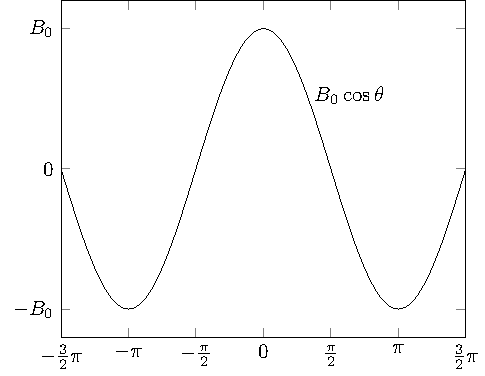
\includegraphics{figBasicFactsCosineWave}
\caption{کوسائن موج}
\label{شکل_حقائق_کوسائن_موج}
\end{figure}
\حصہ{خطی غونډون}
مساوات  \حوالہ{مساوات_بنیادی_سائن_نما_تفاعل} کښ لیکلے شوے چپہ پہ شکل \حوالہ{شکل_حقائق_کوسائن_موج} کښ ښودلے شوے دہ۔دا چپہ \عددیء{2 \pi} ریډیئن اوږدہ دہ او دنګوالے ۓ \عددیء{B_0}  دے۔\عددیء{-\pi/2<\theta<\pi/2} تر مینځہ د دے اوسط دنګوالے د غونډون سرہ داسے حاصلیدے شی۔
\begin{align}\label{مساوات_بنیادی_سائن_نما_تفاعل}
B(\theta)=B_0 \cos \theta
\end{align}
%
\begin{align}
B_{\textup{اوسط}}=\frac{B_0}{\pi}\int_{-\frac{\pi}{2}}^{\frac{\pi}{2}} \cos \theta \dif \theta=\frac{2 B_0}{\pi}
\end{align}
ھم دغہ شان د دغے چپے د مربعے اوسط  مساوات \حوالہ{مساوات_بنیادی_سائن_نما_اوسط_مربع} کښ حاصل کړے شوے دے او د مربعے د اوسط جزر مساوات \حوالہ{مساوات_بنیادی_سائن_نما_اوسط_مربع}  کښ ښودلے شوے دے۔د مربعے د اوسط جزر تہ موثر قیمت وئیلے شی۔
\begin{gather}
\begin{aligned}\label{مساوات_بنیادی_سائن_نما_اوسط_مربع}
B^2_{\textup{اوسط}}&=\frac{B_0^2}{\pi}\int_{-\frac{\pi}{2}}^{\frac{\pi}{2}} \cos^2 \theta \dif \theta\\
&=\frac{B_0^2}{\pi}\int_{-\frac{\pi}{2}}^{\frac{\pi}{2}}\frac{1+\cos 2 \theta}{2} \dif \theta\\
&=\frac{B_0^2}{2}
\end{aligned}
\end{gather}
%
\begin{align}\label{مساوات_بنیادی_سائن_نما_کی_موثر_قیمت}
B_{\textup{موثر}}=\sqrt{B^2_{\textup{اوسط}}}=\frac{B_0}{\sqrt{2}}
\end{align}
\حصہ{سطحی غونډون}
شکل \حوالہ{شکل_حقائق_نلکی_سطحی_تکمل} کښ د دروزے پہ کوږ مخ د \عددیء{B} سطحی کثافت مساوات \حوالہ{مساوات_بنیادی_سائن_نما_تفاعل} کښ ښودلے شوے دے۔راځے چہ د دے دروزے پہ نیم کوږ مخ مثلاً د \عددیء{-\pi/2} او \عددیء{\pi/2} ترمینځ کل مقدار \عددیء{\phi} حاصل کړو۔

مونږ د دروزے پہ کوږ مخ \عددیء{l} اوږدہ او \عددیء{\rho \Delta\theta} پلنہ  وړہ رقبہ \عددیء{\Delta A} اخلو۔نو دغہ رنګ \عددیء{\Delta A} بہ د \عددیء{\rho l \dif \theta} برابر وی او مساوات \حوالہ{مساوات_بنیادی_چوٹے_رقبے_پر_بہاو} مطابق پہ دے وړے سطح بہ  مقدار \عددیء{\Delta \phi} د \عددیء{B \Delta A} برابر وی۔
\begin{figure}
\centering
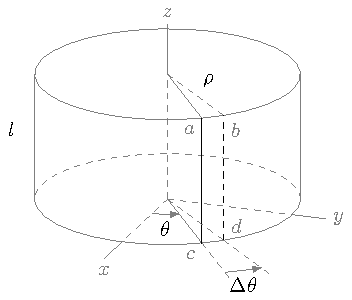
\includegraphics{figBasicFactsCylindricalSurfaceIntegral}
\caption{نلی کی بیرونی سطح پر متغیرہ کا تکمل کُل مقدار دے گی۔}
\label{شکل_حقائق_نلکی_سطحی_تکمل}
\end{figure}
%
\begin{align}\label{مساوات_بنیادی_چوٹے_رقبے_پر_بہاو}
\Delta \phi=B \Delta A=B_0 l \rho \cos \theta \dif \theta
\end{align}
دغہ رنګ د نیم مخ د پارہ مونږ لیکلے شو۔
\begin{align}\label{مساوات_بنیادی_بہاو_بذریع_تکمل_زاویہ_صفر}
\phi = B_0 l \rho \int_{-\pi/2}^{\pi/2} \cos \theta \dif \theta =2 B_0 l \rho
\end{align}
کہ مونږ د دروزے پہ کوږ مخ د \عددیء{(-\pi/2-\alpha)} او \عددیء{(\pi/2-\alpha)} ترمینځ کل مقدار حاصلول غواړو نو د غونډون اول حد بہ ۓ \عددیء{(-\pi/2-\alpha)} شی او آخر حد بہ ۓ \عددیء{(\pi/2-\alpha)} شی۔ لکہ
\begin{align}\label{مساوات_بنیادی_بہاو_بذریع_تکمل_کوئی_زاویہ}
\phi (\alpha) = B_0 l \rho \int_{-\frac{\pi}{2}-\alpha}^{\frac{\pi}{2}-\alpha} \cos \theta \dif \theta =2 B_0 l \rho \cos \alpha
\end{align}
 دلتہ \عددیء{\phi(\alpha)} دا خبرہ ښکارہ کوی چہ نتیجہ پہ \عددیء{\alpha} منحصرہ دہ۔دا یو ډیر اہم مساوات دے۔کہ چرے  دے مساوات کښ الف د صفر برابر واغستے شی نو د دے نہ مساوات \حوالہ{مساوات_بنیادی_بہاو_بذریع_تکمل_زاویہ_صفر} حاصلیږی۔ 
\begin{figure}
\centering
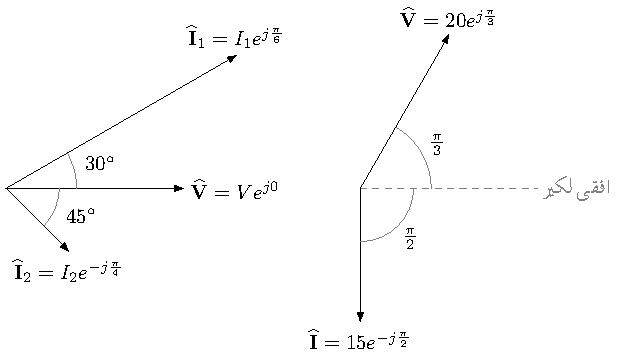
\includegraphics{figBasicFactsPhasors}
\caption{دوری سمتیہ}
\label{شکل_حقائق_دوری_سمتیات}
\end{figure}

\حصہ{دوری سمتیہ}
د نہ بدلیدو تعدد سائن نما چپے  د دوری سمتیے سرہ لیکل ډیر مفید ثابتیږی۔د یولر مساوات
\begin{align}
A_0 e^{\mp j (\omega t + \phi)}=A_0 \cos (\omega t +\phi) \mp j \sin (\omega t+\phi)
\end{align}
مطابق کوسائن چپہ داسے لیکلے شی۔
\begin{align}
A_0 \cos (\omega t +\phi)=\frac{A_0}{2} \left(e^{j(\omega t +\phi)} -e^{-j(\omega t +\phi)}\right)
\end{align}
د دے نہ ثابتیږی چہ کوسائن چپہ دراصل د دوو مخلوط اعدادو مجموعہ دہ۔د یولر مساوات مخلوط عدد ظاہروی چہ پکښ حقیقی جزو کوسائن چپہ او فرضی جزو سائن چپہ وی۔دا رنګے کوسائن چپہ د \عددیء{A_0 e^{j(\omega t +\phi)}} یا \عددیء{A_0 e^{-j(\omega t +\phi)}} حقیقی جزو وی۔رسم دا دے چہ کوسائن چپہ \عددیء{A_0 e^{j(\omega t +\phi)}} لیکلے شی چہ کوم عموماً وړوکی طرز کښ \عددیء{A_0 e^{j\phi}} یا \عددیء{A_0 \phase{\phi}} لیکلے شی۔
دے وړوکی طرز تہ دوری سمتیہ وئیلے شی۔د دوری سمتیہ طول \عددیء{A_0} او زاویہ ئے \عددیء{\phi} وی۔

د دوری سمتیہ استعمالو پہ وخت دا یاد لرے چہ حقیقت کښ دا یو سائن نما چپہ دہ چہ طول ئے \عددیء{A_0}، تعدد ئے \عددیء{\omega} او زاویہ ئے \عددیء{\phi} دہ۔

پہ دے کتاب کښ دوری سمتیہ ظاہرولو دپارہ پہ سادہ لکھائے کښ  د لاطینے ژبے  لوئے حرفونہ چہ پہ سر ئے ټوپے وی استعمال شوی دی، لکہ \عددیء{\hat{I},\hat{V}} او د دوری سمتیے طول ھم پہ دغہ حرف چہ ټوپے پے نہ وی استعمال شوی دی۔دغہ شان برقی دباو \عددیء{v= 20 \cos (\omega t +\frac{\pi}{3})} د پارہ دا ټول لیکلے شی۔
\begin{gather}
\begin{aligned}
v&=20 \cos (\omega t +\frac{\pi}{3})\\
\hat{V}&=20 e^{j \frac{\pi}{3}}\\
\hat{V}&=20 \phase{\frac{\pi}{3}}\\
V&=20\\
\phi&=\frac{\pi}{3}
\end{aligned}
\end{gather}

 د دے مساوات  وړومبی جزو کښ یو کوسائن چپہ پہ عمومی شکل کښ لیکلے شوے دہ۔ھم د دغے چپے دوری شکل پہ دویم او دریم جزونو کښ ښودلے شوے دے۔پہ څلورم جزو کښ ئے طول او پنځم جزو ئے زاویہ ښائی۔
\begin{figure}
\centering
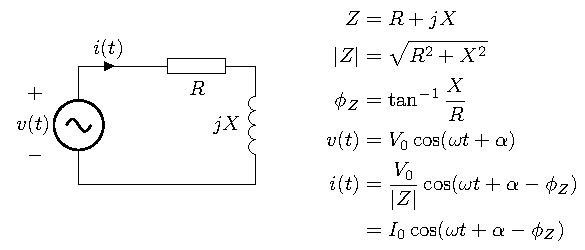
\includegraphics{figBasicFactsRLcircuit}
\caption{دوری سمتیہ کی مدد سے \عددیء{RL} دور کا حل۔}
\label{شکل_حقائق_دوری_سمتیہ_سے_دور_حل}
\end{figure}
دوری سمتیہ ھم د نورو سمتیو پہ شان ګنړلے شی۔دے مساوات کښ د \عددیء{\hat{V}} طول \عددیء{20} دے او  زاویہ یہ \عددیء{\tfrac{\pi}{3}} دہ۔زاویہ د پرتے کرخے  نہ د ګھړے د ستن د چورلیدو  اړولے  اړخ  تہ ناپ کیږی۔پہ شکل \حوالہ{شکل_حقائق_دوری_سمتیات} کښ دا دوری سمتیہ د یو عام سمتیے پہ شان راښکلے شوے دہ۔ پہ دغہ شکل کښ یو څو نورے دوری سمتیے ھم ښو دلے شوی دی۔

برقی دور کښ عموماً د برقی رو زاویہ د برقی دباو پہ نسبت سرہ بیانیږی۔داسے پہ شکل \حوالہ{شکل_حقائق_دوری_سمتیات} کښ \عددیء{\hat{I_1}} برقی رو د برقی دباو نہ دیرش درجہ زاویہ مښکے دہ او برقی رو \عددیء{\hat{I_2}} ترے نہ پنځہ څلویخت درجے زاویہ وروستو دہ۔پہ شکل کښ  \عددیء{45\degree} زاویہ مثبت لیک دہ۔دا زاویہ د پرتے کرخے نہ د ګھړے د ستن چورلیدو اړخ تہ دہ نو ځکہ دا  حقیقت کښ یو منفی زاویہ دہ۔

دے کتاب کښ د ګھړے د ستن د چورلیدو اړولے اړخ تہ د ګھړے اړولے اړخ وئیلے شی او د ګھړے د ستن د چورلیدو اړخ تہ د ګھړے اړخ وئیلے شی۔

راځے چہ د دوری سمتیو سرہ یو برقی دور حل کړو۔داسے بہ ستاسو دوری سمتیے سرہ  پیژنګلو پیدا شی او استعمال بہ ئے ھم ایزدہ کړے۔ 

پہ شکل  \حوالہ{شکل_حقائق_دوری_سمتیہ_سے_دور_حل} کښ  \عددیء{R-L} دور تہ \عددیء{v(t)} برقی دباو ورکړے شوے دہ۔د دوری سمتیو سرہ مونږ برقی رو داسے  حاصلولے شو
\begin{gather}
\begin{aligned}
\hat{I}&=\frac{\hat{V}}{R+j X}=\frac{V_0 \phase{\alpha}}{\abs{Z} \phase {\phi_Z}}\\
&=\frac{V_0}{\abs{Z}} \phase{\alpha-\phi_Z}=I_0 \phase{\alpha-\phi_Z}
\end{aligned}
\end{gather}
 
چہ \عددیء{\phi_Z} پکښ د رکاوټ زاویہ دہ۔دغہ شان سادہ لیک کے برقی رو 
\begin{align}\label{مساوات_بنیادی_حقائق_دوری_سمتیہ_سے_مزاحمت_امالہ_دور_حل}
i(t)=I_0 \cos (\omega t +\alpha-\phi_Z)
\end{align}
حاصلیږی۔
 


